\documentclass[11pt,aspectratio=43,ignorenonframetext,t]{beamer}
% Uses fontspec - assumes compiled with LuaLaTeX or similar
% The above \documentclass is for making slides. If making handouts use:
%\documentclass[11pt,a4paper]{article} 
%\usepackage{beamerarticle}
%\setjobnamebeamerversion{main.beamer}

% See https://github.com/CASSON-LAB/uom_beamer_template
% for details on license, further useage information and similar
%%%%%%%%%%%%%%%%%% DOCUMENT SETUP %%%%%%%%%%%%%%%%%%

% Presentation settings
\mode<presentation>{
  \usetheme[framenumber,titleframestart=1]{UoM_alex}
  \usefonttheme{professionalfonts} % using non standard fonts for beamer
  \usefonttheme{serif}             % set font to Arial
  \usepackage{fontspec}
  \setmainfont[Ligatures=TeX]{Arial}
}

% Handout settings
\mode<article>{
  \usepackage{fullpage}                  % use full page
  \usepackage{fontspec}                  % set font to Arial
    \setmainfont[Ligatures=TeX]{Arial}
  \setlength{\parskip}{1.5\baselineskip} % correct beamer line spacings
  \setlength{\parindent}{0cm}
  \usepackage{enumitem}
    \setlist[itemize]{topsep=0pt}
  \definecolor{uomlinkblue}{HTML}{0071BC}
}


% Packages

% Configurando layout para mostrar codigos C++
\usepackage{listings}
\lstset{
  language=Java,
  basicstyle=\ttfamily\small, 
  keywordstyle=\color{blue}, 
  stringstyle=\color{red}, 
  commentstyle=\color{red}, 
  extendedchars=true, 
  showspaces=false, 
  showstringspaces=false, 
  numbers=left,
  numberstyle=\tiny,
  breaklines=true, 
  backgroundcolor=\color{green!10},
  breakautoindent=true, 
  captionpos=b,
  xleftmargin=0pt,
}

\usepackage{graphicx}  % for graphics files
  \graphicspath{ {./fig/aula6} }
\usepackage{amsmath}   % assumes amsmath package installed
  \allowdisplaybreaks[1] % allow eqnarrays to break across pages
\usepackage{amssymb}   % assumes amsmath package installed 
\usepackage{hyperref} % add hyperlinks to document. Settings are for accessiblity
  \hypersetup{
    colorlinks=true,
    linkcolor=uomlinkblue,
    filecolor=uomlinkblue,      
    urlcolor=uomlinkblue,
	pdflang={en-GB},
}
\usepackage[document]{ragged2e} % left aligned text for accessibility
% experimental - does fundamentally work, if with quite a bit of effort
%\usepackage{axessibility} % LaTeX readable equations for accessibility
%  \tagpdfsetup{tabsorder=structure,uncompress,activate-all,interwordspace=true}
%  \pdfextension catalog{/Lang (en-GB)}
%  \RequirePackage{luacode}
%  \directlua{require("axessibility.lua")}
\usepackage{unicode-math} % unicode maths for accessibility
\usepackage{pdfcomment} % for alt text for accessibility
\usepackage{rotating}  % allow portrait figures and tables
\usepackage{subfigure} % allow matrices of figures
\usepackage{float}     % allows H option on floats to force here placement
\usepackage{multirow}  % allows merging of rows in tables
\usepackage{tabularx}  % allows fixed width tables
\usepackage{ctable}    % modifies \hline for use in table
\usepackage{bm}        % allow bold fonts in equations
\usepackage{pgf}       % allow graphics manipulation
\usepackage{media9}    % allow interactive flash files to be embedded
  \addmediapath{../media}
\usepackage{etoolbox}
  \makeatletter \preto{\@verbatim}{\topsep=0pt \partopsep=0pt} \makeatother  
  
% Custom commands
\newcommand{\matlab}{\emph{\sc{Matlab}}}
\newcommand{\maple}{\emph{\sc{Maple}}}
\newcommand{\simulink}{\emph{\sc{Simulink}}}
\newcommand{\dc}{d.c.}
\newcommand{\ac}{a.c.}
\newcommand{\rms}{RMS}
\newcommand{\wgn}{{\tt wgn}}
\newcommand{\sus}[1]{$^{\mbox{\scriptsize #1}}$}
\newcommand{\sub}[1]{$_{\mbox{\scriptsize #1}}$}
\newcommand{\chap}[1]{Chapter~\ref{#1}}
\newcommand{\sect}[1]{Section~\ref{#1}}
\newcommand{\fig}[1]{Fig.~\ref{#1}}
\newcommand{\tab}[1]{Table~\ref{#1}}
\newcommand{\equ}[1]{(\ref{#1})}
\newcommand{\appx}[1]{Appendix~\ref{#1}}
\newcommand{\degree}{\ensuremath{^\circ}}
\newcommand{\Vrms}{Vrms}
\newcommand{\Vpp}{V\sub{pp}}
\newcommand{\otoprule}{\midrule[\heavyrulewidth]}         
\newcolumntype{Z}{>{\centering\arraybackslash}X}  % tabularx centered columns 
\makeatletter \DeclareRobustCommand{\em}{\@nomath\em \if b\expandafter\@car\f@series\@nil \normalfont \else \bfseries \fi} \makeatother
\newcounter{example_number} % keep track of the example questions



%%%%%%%%%%%%%%%%%% FRONT MATTER %%%%%%%%%%%%%%%%%%
\title{Desenvolvimento de Software}
\subtitle{Aula 8 - Polimorfismo}
\author{Prof. Me. Juliana Costa-Silva}

\begin{document}

\maketitle
%%%%%%%%%%%%%%%%%% TITLE SLIDE %%%%%%%%%%%%%%%%%%
\mode<presentation>{ \frame{\titlepage \label{slide:a}}} 
%\begin{figure}[!ht] 
%\fbox{\includeslide[width=\textwidth]{slide:a}} \end{figure}

%------------------------------------------------------------------------
% \section{Introdução}
 \mode<presentation>{ 
 \begin{frame}{Na última aula...}
 \begin{itemize}
  \item Construtores;
  \item sobrescrita de construtores;
  \end{itemize}
\end{frame}
}
%-------------------------------------------------------------------------
 \mode<presentation>{ 
\begin{frame}
\frametitle{Na aula de hoje...} 
\tableofcontents 
\end{frame}
}

%------------------------------------------------------------------------
% \section{Introdução}
% \begin{frame}{Na última aula...}
%  \begin{itemize}
%   \item Orientação a Objetos;
%   \end{itemize}
% \end{frame}
%-------------------------------------------------------------------------
% \begin{frame}{Dúvidas?}
%  \begin{center}
%    
\includegraphics[height=0.7\paperheight]{duvidas.jpg} \\
%  \end{center}
% \end{frame}
%-------------------------------------------------------------------------------
 \mode<presentation>{\begin{frame}
\frametitle{Na aula de hoje...} 
\tableofcontents 
\end{frame}}
%----------------------------------------------------------------------------
\section{Polimorfismo}
 \mode<presentation>{\begin{frame}{Polimorfismo}{Conceito}
  Polimorfismo (do grego, ``muitas formas'') é a qualidade que permite que uma 
interface acesse uma classe geral de ações. A ação específica é determinada pela 
natureza exata da situação. 
\end{frame}}
%-------------------------------------------------------------------
 \mode<presentation>{\begin{frame}{Polimorfismo}{Exemplo}
  Interface volante.\\
  Independente do mecanismo de direção, a interface não se altera.
  \begin{columns}
    \begin{column}{0.4\textwidth}
      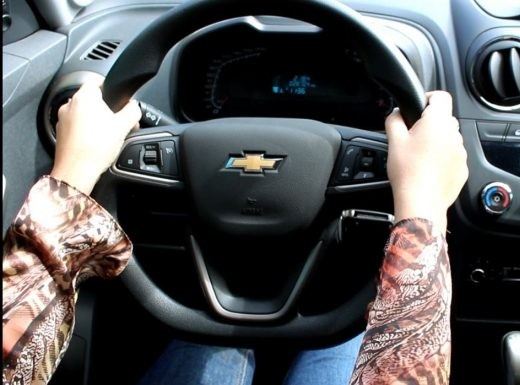
\includegraphics[height=0.3\paperheight]{fig/aula8/volante.jpg}\\
      
    \end{column}
    \pause
    \begin{column}{0.4\textwidth}
        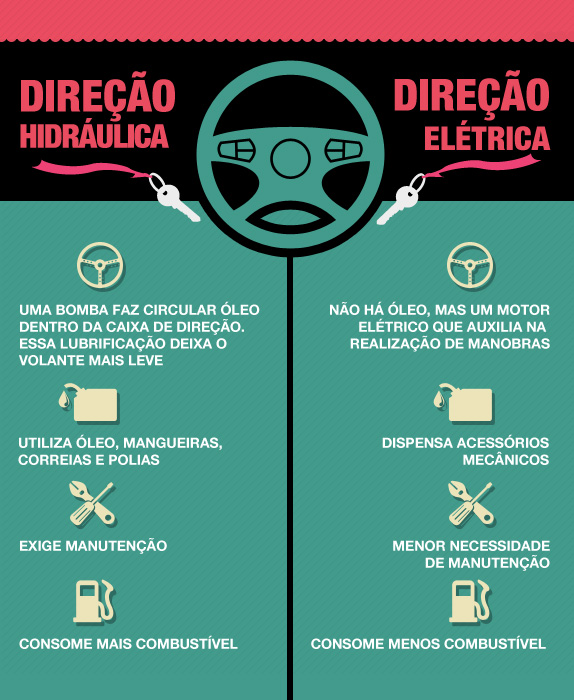
\includegraphics[height=0.5\paperheight]{fig/aula8/direcao.jpg}\\
	
    \end{column}
  \end{columns}
\end{frame}}
%-------------------------------------------------------------------
 \mode<presentation>{\begin{frame}{Polimorfismo}{Exemplo}
    \begin{columns}
    \begin{column}{0.4\textwidth}
      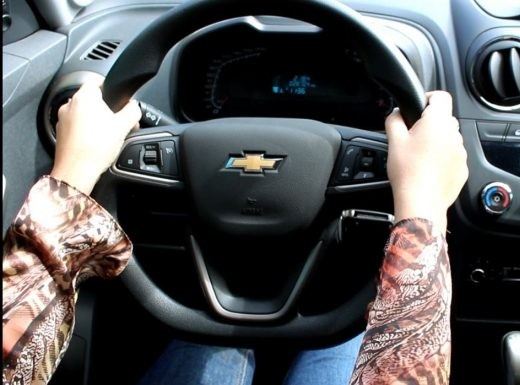
\includegraphics[height=0.3\paperheight]{fig/aula8/volante.jpg}\\    
    \end{column}
    \pause
    \begin{column}{0.4\textwidth}
        \begin{itemize}
          \item O volante funciona da mesma forma;
	  \pause \item A maneira de utilizar será igual;
	  \pause \item Se você souber operar o volante poderá dirigir carros 
com direção elétrica, hidráulica ou manual.
         \end{itemize}
    \end{column}
  \end{columns}
\end{frame}}
%-------------------------------------------------------------------
 \mode<presentation>{\begin{frame}{Polimorfismo}{Exemplo Programação}
  \begin{itemize}
    \item Criamos um programa que simula o movimento de vários animais para um 
estudo biológico. 
    \pause \item As classes \textbf{Peixe, Anfibio} e \textbf{Passaro} 
representam três tipos de animais sob investigação.
    \pause \item Cada tipo de  \textbf{Animal} responde a uma mensagem mover de 
uma maneira única (peixe nada um metro, anfíbio pula um metro, pássaro voa um 
metro)
    \pause \item Cada objeto, sabe como se movimentar a sua maneira.
  \end{itemize}
\end{frame}}
%-------------------------------------------------------------------
 \mode<presentation>{\begin{frame}{Polimorfismo}{Exemplo Programação - II}
  \begin{itemize}
    \item Para simular os movimentos dos animais, o programa envia a mesma 
mensagem a cada objeto (\textcolor{purple}{mover});
    \pause \item Toda subclasse implementa o método \textit{mover}.
    \pause \item O nosso programa mantém um array de \textbf{Animal}.
    \pause \item Sempre que necessitamos executar um movimento em um animal 
qualquer, chamaremos o mesmo método: \textcolor{purple}{mover}
    \pause \item Entretanto, cada animal se move de maneira diferente.
  \end{itemize}
\end{frame}}
%----------------------------------------------------------------------------
 \mode<presentation>{\section{Implementando Polimorfismo}
\begin{frame}{Animal.java}
  Implemente a classe Animal.
  \tiny
  \begin{block}{Atributos}
   \begin{itemize}
    \item nome
    \item patas
    \item velocidade
    \item localizacao
   \end{itemize}
  \end{block}
  \begin{block}{Métodos}
   \begin{itemize}
     \item Construtor
     \item mover() (mostra o ``rastro'' do animal)
    \item Getters e Setters
   \end{itemize}
  \end{block}

\end{frame}}
%----------------------------------------------------------------------------
 \mode<presentation>{\begin{frame}{Animal.java}
 \small{ 
\lstinputlisting[linerange={3-20}]{cod/aula8/Animal.java}}
\end{frame}}
%----------------------------------------------------------------------------
 \mode<presentation>{\begin{frame}{Peixe.java}
  Implemente a classe Peixe.
  \tiny
  \begin{block}{Atributos}
   \begin{itemize}
    \item nome
    \item patas
    \item velocidade
    \item localizacao
    \item agua //0 = doce, 1 = salgada
   \end{itemize}
  \end{block}
  \begin{block}{Métodos}
   \begin{itemize}
     \item Construtor
     \item mover() (mostra o ``rastro'' do animal)
    \item Getters e Setters
   \end{itemize}
  \end{block}

\end{frame}}
%----------------------------------------------------------------------------
 \mode<presentation>{\begin{frame}{Peixe.java}
 \small{ 
\lstinputlisting[linerange={3-17}]{cod/aula8/Peixe.java}}
\end{frame}}
%----------------------------------------------------------------------------
 \mode<presentation>{\begin{frame}{Passaro.java}
  Implemente a classe Passaro.
  \tiny
  \begin{block}{Atributos}
   \begin{itemize}
    \item nome
    \item patas
    \item velocidade
    \item localizacao
   \end{itemize}
  \end{block}
  \begin{block}{Métodos}
   \begin{itemize}
     \item Construtor
     \item mover() (mostra o ``rastro'' do animal)
    \item Getters e Setters
   \end{itemize}
  \end{block}

\end{frame}}
%----------------------------------------------------------------------------
 \mode<presentation>{\begin{frame}{Passaro.java}
 \small{ 
\lstinputlisting[linerange={3-17}]{cod/aula8/Passaro.java}}
\end{frame}}
%----------------------------------------------------------------------------
 \mode<presentation>{\begin{frame}{Anfibio.java}
  Implemente a classe Anfibio.
  \tiny
  \begin{block}{Atributos}
   \begin{itemize}
    \item nome
    \item patas
    \item velocidade
    \item localizacao
   \end{itemize}
  \end{block}
  \begin{block}{Métodos}
   \begin{itemize}
     \item Construtor
     \item mover() (mostra o ``rastro'' do animal)
    \item Getters e Setters
   \end{itemize}
  \end{block}

\end{frame}}
%----------------------------------------------------------------------------
 \mode<presentation>{\begin{frame}{Anfibio.java}
 \small{ 
\lstinputlisting[linerange={3-17}]{cod/aula8/Anfibio.java}}
\end{frame}}
%----------------------------------------------------------------------------
 \mode<presentation>{\begin{frame}{ClassePrincipal.java}
  Implemente a classe Classe Principal.
  \tiny
  \begin{block}{Execução}
   \begin{itemize}
    \item Conter um array de objetos Animal;
    \item Adicionar ao array: Passaro, Peixe e Anfibio;
    \item Executar o método mover em um laço de repetição.
   \end{itemize}
  \end{block}
  \begin{block}{Métodos}
   \begin{itemize}
     \item main()
   \end{itemize}
  \end{block}

\end{frame}}
%----------------------------------------------------------------------------
 \mode<presentation>{\begin{frame}{Aula13.java}
 \small{ 
\lstinputlisting[linerange={8-23}]{cod/aula8/Aula8.java}}
\end{frame}}
%----------------------------------------------------------------------
\section{Atividade}
 \mode<presentation>{
\begin{frame}{Atividade - Relembrando}
  \small
  \begin{enumerate}
   \item Crie uma classe Conta, que possua um saldo, e os métodos para pegar 
saldo, depositar, e sacar.
    \item Crie os métodos get e set para cada atributo.
    \item Adicione um método na classe Conta, que atualiza o saldo da conta de 
acordo com uma taxa percentual fornecida.
    \item Crie duas subclasses da classe Conta : ContaCorrente e ContaPoupanca. 
Ambas terão o método atualiza reescrito: A ContaCorrente deve atualizar-se com o 
dobro da taxa e a ContaPoupanca deve atualizar-se com o triplo da taxa.
    \item Além disso, a ContaCorrente deve reescrever o método deposita, afim 
de retirar uma taxa bancária de dez centavos de cada depósito.
    \item Crie uma classe com método main e instancie essas classes, atualize-as 
e veja o resultado.
  \end{enumerate}
\end{frame}}
%-----------------------------------------------------------------------
\section{Leitura recomendada}
 \mode<presentation>{\begin{frame}{Leitura complementar}
 Para mais informações sobre JAVA, leia:\\
 \begin{columns}
   \begin{column}{0.4\textwidth}
     Java: Como programar\\
     Capítulo 10:\\ 
      \cite{deitel2017java}
   \end{column}
   \begin{column}{0.3\textwidth}
    \begin{center}
  
\includegraphics[height=0.5\paperheight]{fig/aula1/deitel2017java.png} \\
 \end{center}
   \end{column}
 \end{columns}
\end{frame}}
%----------------------------------------------------------------------------------------------------------------------
 
 \mode<presentation>{\begin{frame}{Referências}%[allowframebreaks]
 \small
 \begin{center}
 	\bibliographystyle{apalike}
	 \bibliography{ref_aula_progI}
 \end{center}
 \end{frame}}

\begin{figure}[!ht] \fbox{\includeslide[width=\textwidth]{slide:z}} \end{figure}
Text for notes goes here. 
\begin{itemize}
  \item List 1. 
  \item List 2. 
\end{itemize}


%%%%%%%%%%%%%%%%%% END MATTER %%%%%%%%%%%%%%%%%%
\end{document}